\documentclass[tikz,border=2pt]{standalone}
\usepackage{amsmath}
\usepackage{pgfplots}
\pgfplotsset{compat=1.18}
\usetikzlibrary{arrows.meta}
\begin{document}
% Example 1: f(x)=3x^2 on the non-convex V=[-2,1] u [2,3]: local minimum on V at x=2 with f(2)=12,
% global minimum on V at x=0 with f(0)=0; the chord from (2,12) to (0,0) runs over the gap (1,2), which is not in V.
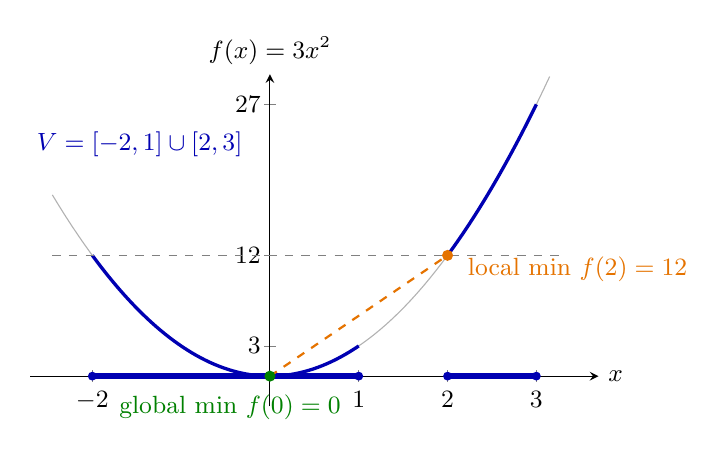
\begin{tikzpicture}[font=\small, >={Latex[length=2mm]}]
  \begin{axis}[
    axis lines=middle, xmin=-2.7, xmax=3.7, ymin=-3, ymax=30,
    xtick={-2,1,2,3}, ytick={3,12,27},
    xlabel={$x$}, ylabel={$f(x)=3x^2$},
    xlabel style={anchor=west}, ylabel style={anchor=south},
    width=8.8cm, height=5.8cm, clip=false,
    yticklabel style={fill=white, inner sep=1pt}
    ]
    \addplot[gray!60, thin, domain=-2.45:3.15, samples=80] {3*x^2};
    \addplot[blue!70!black, very thick, domain=-2:1, samples=60] {3*x^2};
    \addplot[blue!70!black, very thick, domain=2:3, samples=30] {3*x^2};
    \draw[blue!70!black, line width=2.2pt] (axis cs:-2,0) -- (axis cs:1,0) (axis cs:2,0) -- (axis cs:3,0);
    \fill[blue!70!black] (axis cs:-2,0) circle (1.6pt) (axis cs:1,0) circle (1.6pt) (axis cs:2,0) circle (1.6pt) (axis cs:3,0) circle (1.6pt);
    \node[blue!70!black, anchor=east] at (axis cs:-0.2,23) {$V=[-2,1]\cup[2,3]$};
    \draw[gray, thin, dashed] (axis cs:-2.45,12) -- (axis cs:3.3,12);
    \draw[orange!90!black, thick, dashed] (axis cs:0,0) -- (axis cs:2,12);
    \fill[orange!90!black] (axis cs:2,12) circle (2pt);
    \node[orange!90!black, anchor=west] at (axis cs:2.12,10.6) {local min $f(2)=12$};
    \fill[green!50!black] (axis cs:0,0) circle (2pt);
    \node[green!50!black, anchor=north] at (axis cs:-0.45,-0.9) {global min $f(0)=0$};
  \end{axis}
\end{tikzpicture}
\end{document}
